%&program=xelatex
%&encoding=UTF-8 Unicode
% SVN keywords
% $Author$
% $Date$
% $Revision$
% $URL$
\documentclass[a4paper,twoside,12pt]{article}      % Comments after  % are ignored
%\usepackage{hyperref}                 % For creating hyperlinks in cross references
%
\usepackage{ifxetex}% for XELATEX, or PDFlatex
\usepackage{ifplatform} 
%
\ifxetex
	\usepackage{polyglossia} \setmainlanguage{portuges}
	\usepackage{fontspec}
	\ifwindows
		\setmainfont[Ligatures=TeX]{Garamond}
		\setsansfont[Ligatures=TeX]{Gill Sans MT}
%	\setmonofont[Scale=MatchLowercase]{Courier}
		\setmonofont[Scale=0.95]{Courier}
	\fi
	\iflinux
		\setmainfont[Ligatures=TeX]{Linux Libertine O}
		\setsansfont[Ligatures=TeX,Scale=MatchLowercase]{Linux Biolinum}
		\setmonofont[Scale=MatchLowercase]{Courier}
	\fi
	\ifmacosx
	% add settings
	% Use xelatex -no-shell ...
	\fi
	\usepackage{xcolor,graphicx} 
\else
	\usepackage[portuguese]{babel}
	%\usepackage[latin1]{inputenc}
	\usepackage[utf8]{inputenc}
	\usepackage[T1]{fontenc}
	\usepackage{graphics}                 % Packages to allow inclusion of graphics
	\usepackage{color}                    % For creating coloured text and background
\fi

\usepackage{amsmath,amssymb,amsfonts} % Typical maths resource packages
\usepackage{multicol}

\oddsidemargin 0cm
\evensidemargin 0cm

\pagestyle{myheadings}         % Option to put page headers
                               % Needed \documentclass[a4paper,twoside]{article}
\markboth{{MEFT}}
{{\small\it \protect\input{../../LIFE.txt}}}

\textwidth 15.5cm
\topmargin -1cm
\parindent 0.5cm
\textheight 24cm
\parskip 1mm

\usepackage{enumitem}
\setlist{nolistsep}

%\usepackage{textcomp}

% Math macros
\newcommand{\ud}{\,\mathrm{d}} 
\newcommand{\HRule}{\rule{\linewidth}{0.5mm}}

\author{Prof. Bernardo B. Carvalho} 

%, Bernardo Brotas Carvalho\\bernardo@ipfn.ist.utl.pt} 
\date{ Setembro 2014} 

\begin{document} 


\includegraphics[width=0.2\textwidth]{../../logo-ist}%\\[1cm]  %%  Logo_IST_color

\HRule \\[0.5cm]
{ \large   \bfseries \textsc{ Experiência de Thomson. Determinação experimental da relação $q/m$ do electrão }}\\
\HRule \\%[0.5cm]

\section{\sf OBJECTIVO DO TRABALHO}
Pretende-se com este trabalho determinar a relação entre a carga e a massa ($q/m$) do electrão. Para esse fim, vamos estudar a deflexão de um feixe de raios catódicos sob o efeito simultâneo de um campo eléctrico e de um campo magnético.

Os raios catódicos foram inventados em 1879 por William Crookes (1832--1919), mas foi Sir J. J. Thomson\footnote{Prémio Nobel da Física de 1906, em reconhecimento dos seus trabalhos teóricos e experimentais na condução da electricidade em gases.} (1856--1940) que, em 1897, relatou as experiências por si realizadas e que permitiram determinar o valor daquela relação. Além disso, estas experiências provaram que os raios catódicos são constituídos por partículas de carga negativa, desde então designadas por electrões. Neste trabalho iremos reproduzir aproximadamente a experiência de Thomson.

\section{\sf INTRODUÇÃO TEÓRICA}
\subsection{\sf  Conceitos necessários:} 
\begin{enumerate}
	\item Força eléctrica. Campo eléctrico (Electrostático).
	\item Potencial eléctrico. Equipotencial. Energia potencial eléctrica.
	\item Condutores e dieléctricos. Condensador plano.
	\item Efeitos da corrente eléctrica estacionária criada por uma espira. 	
	\item Força de Lorentz e Laplace.
\end{enumerate}

\subsection{\sf Campo electrostático}

Define-se como sendo o campo eléctrico criado por uma distribuição de cargas que \emph{não evolui no tempo}. Considere-se por exemplo o par de cargas $q_1$ e $q_2$ imersas no vácuo, à distância $r_{12}$, e situadas respetivamente em $P_1$ e $P_2$, conforme ilustrado na Fig. \ref{fig:fig1}. A força eléctrica que sofre $q_1$ no ponto $P_1$ devido a $q_2$ em $P_2$ à distância $r_{12}$ é
\begin{equation}
	\vec{F}_{P_1,q_1} (q_2, r_{1 2} ) = \frac{q_1 q_2}{4 \pi \varepsilon_0 r_{1 2}^2} \vec{u}_{r,P_1} = 
	- \vec{F}_{P_2,q_2} (q_1, r_{1 2} )
%	B = \mu H \to H= \sqrt{\frac{ \varepsilon}{\mu}} E 
\end{equation}
em que $\varepsilon_0$  é designada por constante dieléctrica ou permitividade eléctrica do vazio ($\varepsilon_0 \simeq 8.854 \cdot 10^{-12}$ F/m) e	
 $\vec{u}_{r,P_1}$  é o \emph{versor} da distância $r_{1 2} $ no ponto $P_1$  (vector unitário dirigido de $P_2$ para $P_1$, ver figura).

%\begin{minipage}[b]{0.5\linewidth}
Define-se campo eléctrico $\vec{E}$  num ponto $P$, criado por uma carga $q_1$ à distância $r$, como a força eléctrica que se exerce em $P$  devido à carga $q_1$ sobre uma carga de prova ou teste, suposta unitária e positiva:
\begin{equation}
	\vec{E}_P (q_1, r) = \frac{q_1}{4 \pi \varepsilon_0 r^2} \vec{u}_{r, P} 
\end{equation}

\begin{figure}[tb]
  \centering 
	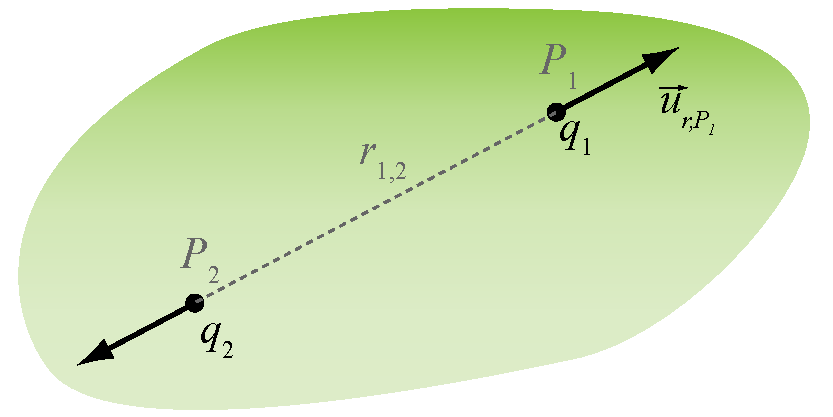
\includegraphics[width=0.6\textwidth]{./fig1-thomson} 
	\caption{ Definição dos termos para a geometria de duas cargas. \label{fig:fig1}} 

\end{figure}
%\end{minipage}
%\hspace{0.1cm}
%				\begin{minipage}[b]{0.5\linewidth}
%				\setlength{\unitlength}{1.0cm} 
%				\begin{picture}(6,6)
%				\linethickness{0.075mm} 
%				\put(1,1){\line(1,1){4}}
%				\put(1,1){\circle*{0.1}}
%				\put(5,5){\circle*{0.1}}
%
%				\put(.8,1.4){$P_2$}
%				\put(1.2,.7){$q_2$}
%				\put(4.8,5.4){$P_1$}
%				\put(5.2,4.7){$q_1$}
%				\put(3.6,3.0){$r_{12}$}
%				\put(5.4,5.3){$\vec{u}_{r,P_1}$}
%				%\linethickness{1.1mm} 
%				\thicklines
%				\put(5,5){\vector(1,1){0.8}}
%				\put(1,1){\vector(-1,-1){0.8}}
%				\end{picture}
%				\end{minipage}
As linhas de força eléctrica geradas por $q_1$ são radiais e dirigidas para o exterior, se $q_1>0$, ou para a origem, se $q_1<0$. Se se colocasse em $P$  a carga $q$,  a força eléctrica a que esta carga ficaria submetida devido a $q_1$  seria	
$\vec{F}_{P,q} (q_1, r ) = q \vec{E}$, 
ou mais simplesmente:
\begin{equation}
\vec{F} = q \vec{E}
\end{equation}

A expressão ``campo eléctrico" também define a região do espaço onde se fazem sentir as acções eléctricas.

\subsection{\sf Potencial eléctrico}
	
O campo eléctrico e a força eléctrica, que são entidades vetoriais, podem também ser calculadas a partir de uma entidade capaz de descrever o campo mas de natureza escalar, o potencial eléctrico $V$. Para a situação referida acima, o potencial eléctrico criado no ponto $P$ à distância $r$ da carga $q_1$ é calculado por:
\begin{equation} \label{eq:pot_ele}
	V_P (q_1, r) = \frac{q_1}{4 \pi \varepsilon_0 r} 
\end{equation}


No caso de uma distribuição de $n$ cargas eléctricas $q_i$ à distância $r_i$ do ponto $P$ onde se pretende calcular o campo eléctrico e o potencial, tem-se:
\begin{align}
	\vec{E}_P &= \frac{1}{4 \pi \varepsilon_0 } \sum_{i=1}^n \Big( \frac{q_i}{ r_i^2}\; \vec{u}_{r_i , P}  \Big) \nonumber \\ 
 V_P &= \frac{1}{4 \pi \varepsilon_0 } \sum_{i=1}^n \Big( \frac{q_i}{ r_i}  \Big) \nonumber
\end{align}

%\setlength{\unitlength}{0.8cm} 
%\begin{picture}(6,4)
%\linethickness{0.075mm} \multiput(0,0)(1,0){7}
%{\line(0,1){4}} \multiput(0,0)(0,1){5}
%{\line(1,0){6}} \thicklines \put(0.5,0.5){\line(1,5){0.5}} \put(1,3){\line(4,1){2}} \qbezier(0.5,0.5)(1,3)(3,3.5) \thinlines %\put(2.5,2){\line(2,-1){3}} \put(5.5,0.5){\line(-1,5){0.5}} \linethickness{1mm} \qbezier(2.5,2)(5.5,0.5)(5,3) \thinlines %\qbezier(4,2)(4,3)(3,3) \qbezier(3,3)(2,3)(2,2) \qbezier(2,2)(2,1)(3,1) \qbezier(3,1)(4,1)(4,2)
%\end{picture}


Recorde-se que se se considera uma única carga $q_1$ positiva, as linhas de força eléctricas são radiais e dirigidas para o exterior. Essas linhas de força são perpendiculares às \emph{superfícies equipotenciais}, que são esféricas ($r = \mathrm{c.^{te}}$ na equação \ref{eq:pot_ele}) e concêntricas com as cargas. Atendendo a (\ref{eq:pot_ele}) para dois raios $r_1$ e $r_2$ tal que $r_2 > r_1$ temos $V(r_2) < V(r_1)$, e portanto as linhas de força dirigem-se para os potenciais decrescentes.

Considere-se agora o caso de duas cargas $q_1 > 0$ e $q_2 < 0$. Enquanto estiverem muito afastadas uma da outra, produzem campos radiais, respetivamente divergindo e convergindo. Se forem colocadas suficientemente próximas, as linhas de força vão sofrer a influência de ambas as cargas. Nesse caso, há uma única linha de força que é linear, dirigida de $q_1$ para $q_2$. Todas as outras, que na vizinhança próxima de cada carga são radiais, acabam por infletir, dirigindo-se de $q_1$ para $q_2$. A figura das linhas de força tem simetria de revolução em torno do eixo que contém $q_1$ e $q_2$ e é esquematicamente a indicada na figura \ref{fig:sup-equip}. Se o valor absoluto das duas cargas for o mesmo a figura é simétrica em relação ao plano mediatriz das cargas $q_1$ e $q_2$ \footnote{Para mais exemplos ver http://www.flashphysics.org/electricField.html}.

\begin{figure}[tb]
  \centering 
	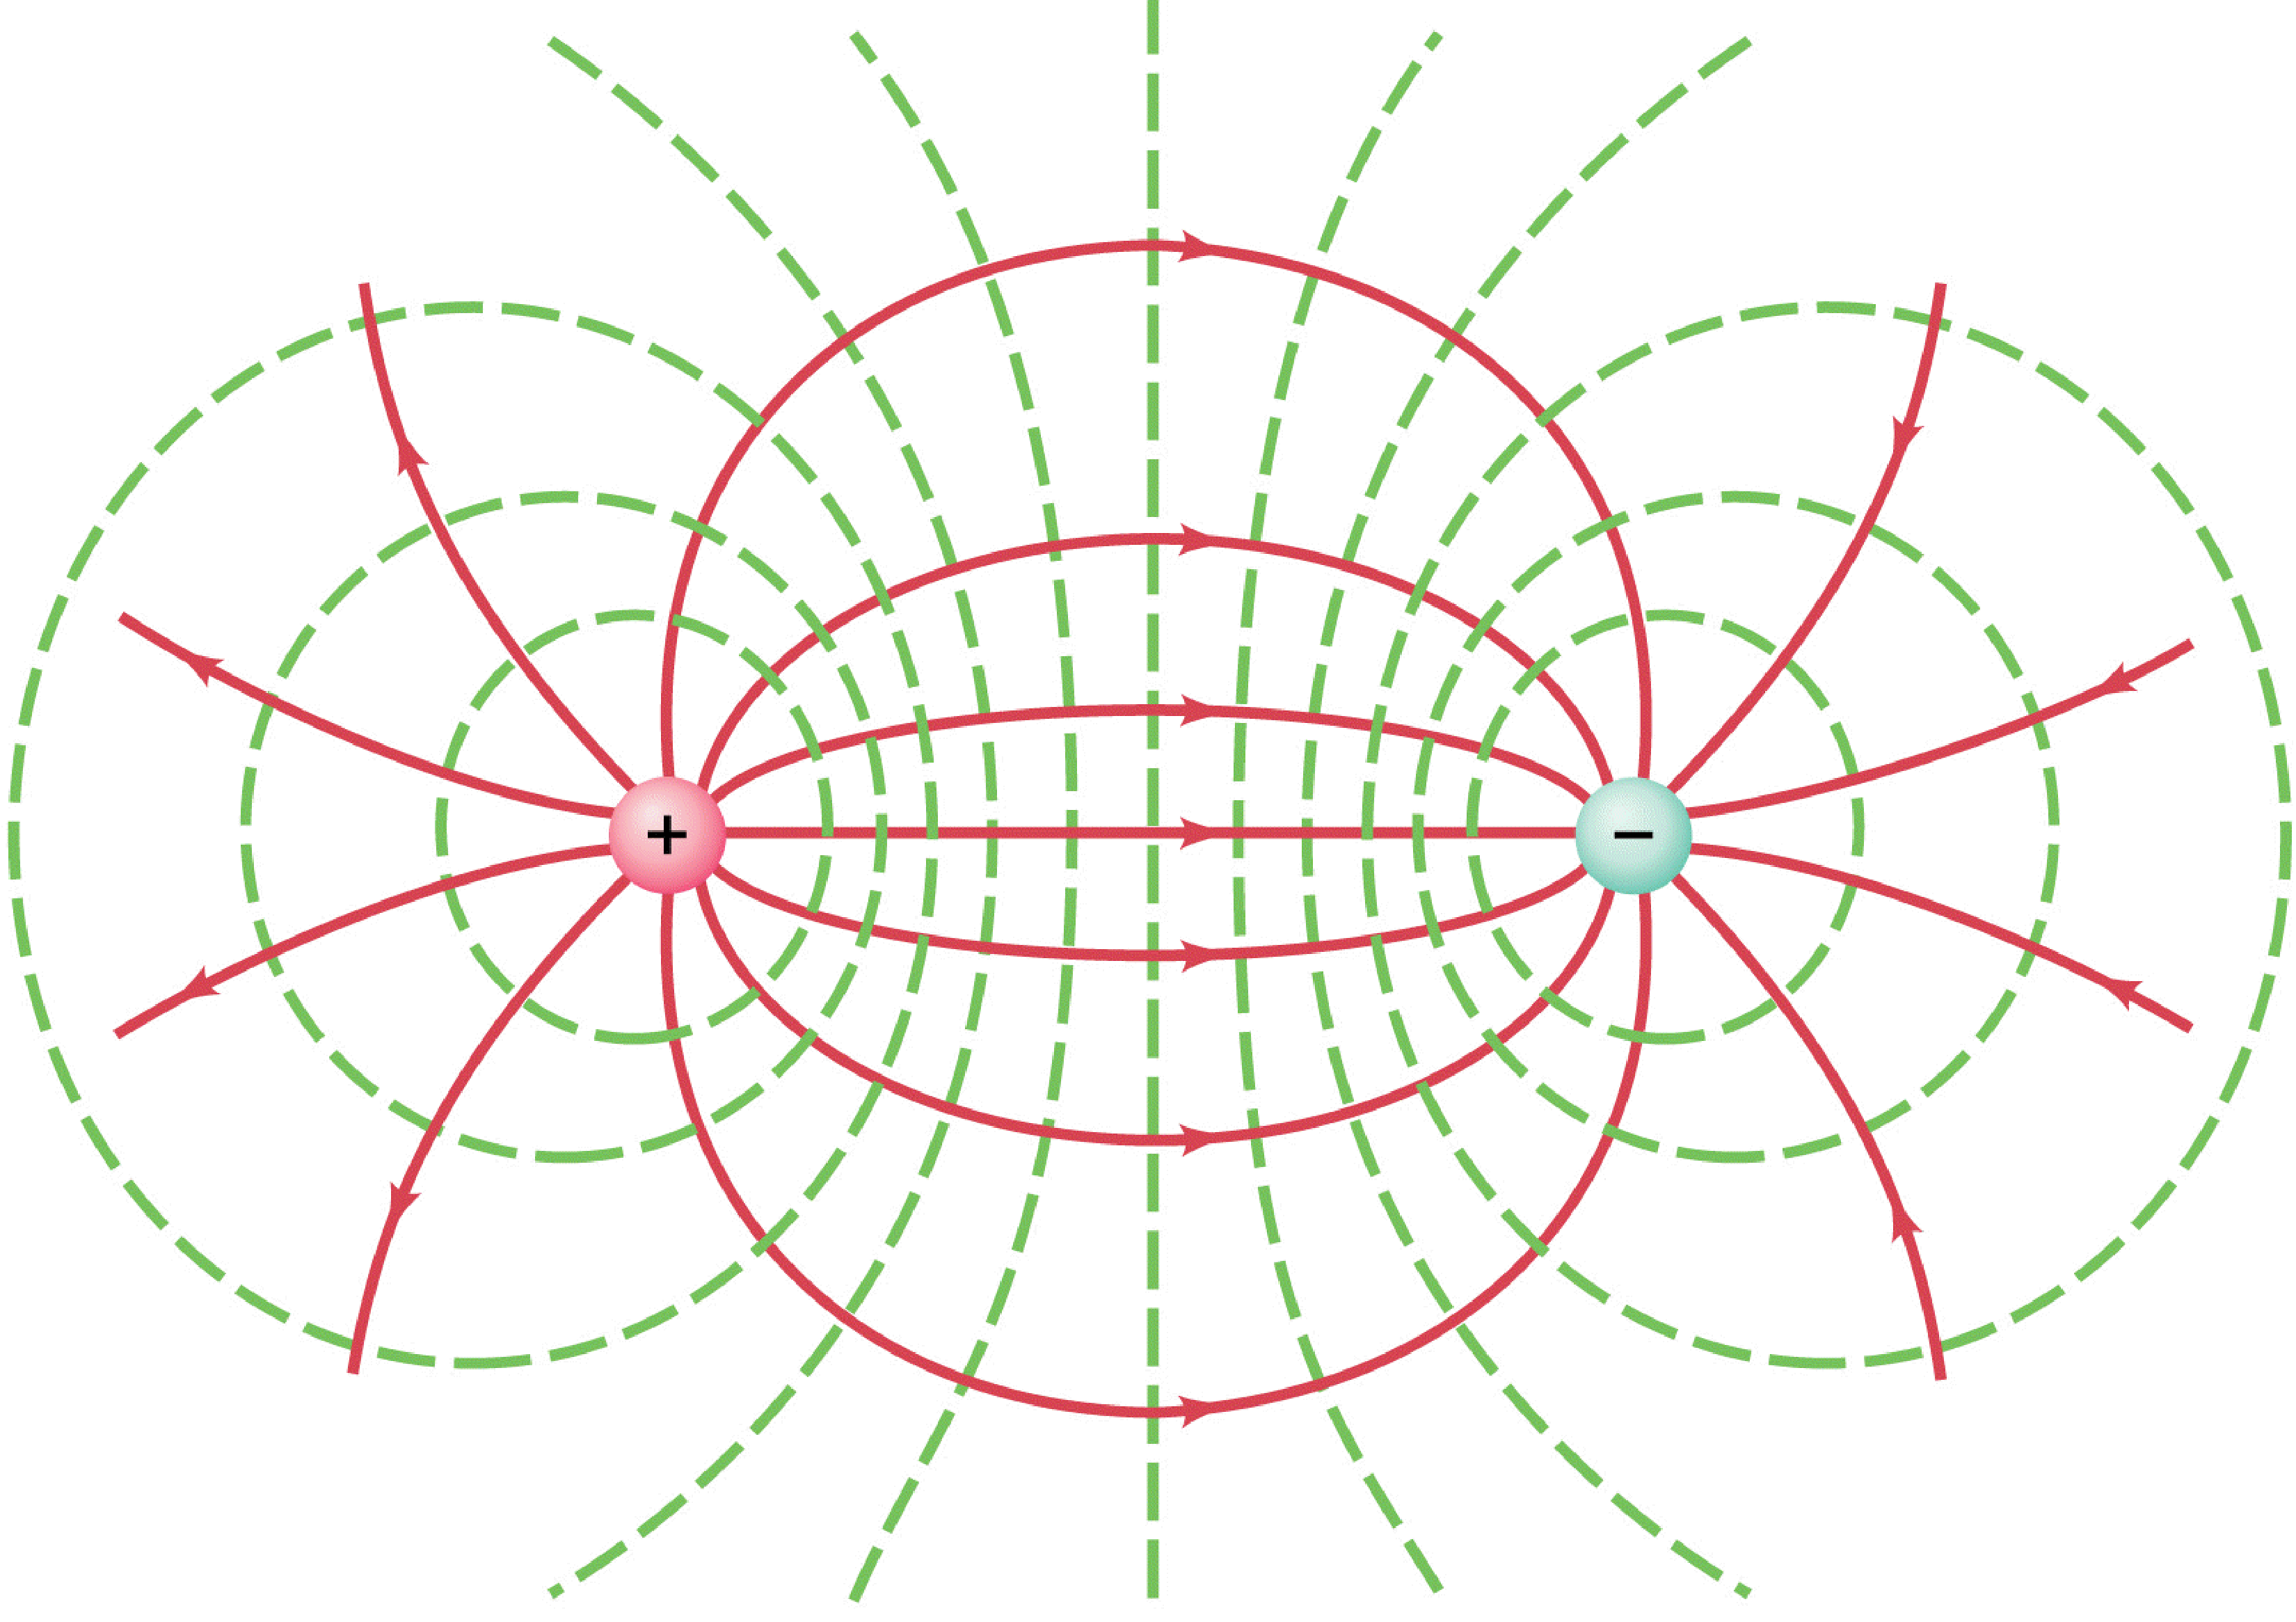
\includegraphics[width=0.5\textwidth]{./fig2-thomson} 
	\caption{ Linhas de força (a vermelho) e superfícies equipotenciais (a verde) de duas cargas simétricas. \label{fig:sup-equip}} 
\end{figure}

Se se calcular a diferença de potencial entre dois pontos infinitamente próximos $P$ e $P+dP$ devida a uma carga $q_1$ à distância $r$ e $r+dr$ respetivamente, a variação elementar do potencial $V$ será:
%\begin{minipage}[b]{0.45\linewidth}
\begin{align}
d V &= V_{P+dP} - V_P = \frac{q_1}{4 \pi \varepsilon_0 r} \big(  \frac{1}{r + dr} -\frac{1}{r} \big)\nonumber\\
	 &\approx \frac{q_1}{4 \pi \varepsilon_0 } \big(  - \frac{dr}{r^2} \big) = - \vec{E} \cdot d \vec{r}  \end{align}
%\end{minipage}
%
%\hspace{0.1cm}
%
%\begin{center}
%\begin{minipage}[b]{0.6\linewidth}
%\framebox[0.6\linewidth][c]{
%\setlength{\unitlength}{0.8cm} 
%\begin{picture}(6,4)
%\linethickness{0.075mm} \multiput(0,0)(1,0){7}
%{\line(0,1){4}} \multiput(0,0)(0,1){5}
%{\line(1,0){6}} \thicklines \put(0.5,0.5){\line(1,5){0.5}} \put(1,3){\line(4,1){2}} \qbezier(0.5,0.5)(1,3)(3,3.5) \thinlines %\put(2.5,2){\line(2,-1){3}} \put(5.5,0.5){\line(-1,5){0.5}} \linethickness{1mm} \qbezier(2.5,2)(5.5,0.5)(5,3) 
%\put(1,2){\circle*{0.15}}
%\put(5,2){\circle*{0.15}}
%\put(.8,0.8){$q_1 (+)$}
%\put(4.8,0.8){$q_2 (-)$}
%\thinlines 
%\qbezier(1.15,2.15)(3,4)(4.9,2.1) 
%\qbezier(1.1,2.1)(3,3)(4.9,2.1) 
%\put(4.5,2.5){\vector(1,-1){0.4}}
%\qbezier(1.1,1.9)(3,1)(4.9,2)
%\put(4.9,1.9){\vector(1,1){0.4}}


%\qbezier(1.2,2.2)(3,3.5)(4.8,2.2) 
%\put(4.8,2.2){\vector(1,-1){0.3}}
%\qbezier(1.2,1.8)(3,.5)(4.8,1.8)
%\put(4.5,1.5){\vector(1,1){0.4}}

%\put(.9,2){\vector(-1,0){.8}} 
%\put(1.1,2){\vector(1,0){3.7}} 
%\put(5.9,2){\vector(-1,0){.8}} 
%\qbezier(2,2)(2,1)(3,1) \qbezier(3,1)(4,1)(4,2)
%\end{picture}
%\end{minipage}

%\setlength{\unitlength}{1mm} 
%\begin{picture}(60,40)
 
%\put(10,20){\circle*{0}}
%\put(50,20){\circle*{0}}
%\qbezier(11.5,21.5)(30,40)(49,21) 
%\put(45,25){\vector(1,-1){1}}
%\put(45,25){\vector(1,-1){2}}
%\end{picture}

Esta quantidade representa o trabalho elementar (energia) associado ao deslocamento da
carga teste ($q_t=1\,$ C), de $P$ para $P+dP$. Para $q_1 > 0$,	$\vec{E}$ e $\vec{dr}$ são paralelos e $dV < 0$. Isto significa que
não será necessário fornecer energia para realizar esse transporte. 
De facto, afastar a carga teste da carga $q_1$ (i.e. ir de $P$ para $P+dP$) leva a uma configuração de cargas ($q_1$ e $q_t$) energeticamente mais favorável \footnote{Recorde-se que para um campo conservativo o trabalho realizado (que não depende do percurso mas só dos pontos inicial e final) tem um valor simétrico da variação de energia potencial.}.

No caso de uma diferença finita de potencial, isto é de uma diferença de potencial entre dois pontos $P$ e $Q$, ter-se-á que somar um número infinito de contribuições infinitesimais $dV_i=- \vec{E}_i \cdot d\vec{r}_i$ no intervalo de $P$ a $Q$:

\begin{equation}
V_Q-V_P  = \lim_{n  \to \infty } \sum_{i=1}^n dV_i = \lim_{n \to \infty } \sum_{i=1}^n \underbrace{( - \vec{E}_i \cdot d\vec{r}_i )}_{\overline{PQ}} \rightarrow \int - \vec{E} \cdot d\vec{r}
\end{equation}
%\frown 

\begin{equation*} 
V_P - V_Q  = \int_{\overline{PQ}}  \vec{E} \cdot d \vec{r}
\end{equation*}
e porque $\vec{E}$ (campo electrostático) é um campo conservativo, este integral não vai depender do percurso mas apenas dos pontos extremos, i.e.
\begin{equation*} 
V_P - V_Q  = \int_P^Q  \vec{E} \cdot d\vec{r}
\end{equation*}


No caso particular de $E$ ser homogéneo (por exemplo no interior de um condensador plano)  na região onde se situam os pontos $P$ e $Q$, afastados de uma distância $D$, obtém-se 
\begin{equation}\label{eq:difPot}
V_P - V_Q  =  \vec{E}\cdot\vec{PQ}=E\cdot D
\end{equation}

Para se compreender o significado físico de $V_P$, imagine-se que $Q$ é um ponto infinitamente
afastado da região em que se faz sentir o campo eléctrico $\vec{E}$.
Nesse ponto, $r \to \infty $ e $V_Q=0$,
obtendo-se $V_P =  \int_P^\infty  \vec{E} \cdot d\vec{r}$, que permite a seguinte interpretação:
\newline
\newline
\fbox {\begin{minipage}{35em}
O potencial eléctrico $V_P$ é a energia necessária para transportar a carga-teste, sob acção de $\vec{E}$, desde o ponto $P$ até uma distância suficientemente grande tal que o campo eléctrico não se faça sentir.
\end{minipage}}
\newline
\newline
Assim, $V$ tem sempre o significado de uma diferença de potencial.

%Se for a carga $q_2$, a energia necessária será $W= q_2\cdot V$. 
\subsection{{\sf Energia electrostática}}
A energia associada a uma configuração de cargas $q_1$ e $q_2$, à distância $r$, é dada por:

\begin{equation}\label{eq:enrPot}
 W = \frac{q_1 q_2}{4 \pi \varepsilon_0 r} = q_1 V_1 = q_2 V_2 =  \frac{q_1 V_1 +q_2 V_2}{2} 
\end{equation}
em que $V_1$ é o potencial no ponto $P_1$ criado pela carga $q_2$, e $V_2$ é o potencial no ponto $P_2$ criado pela carga $q_1$. 

Recordando a definição do potencial criado por $n$ cargas eléctricas, podemos generalizar a equação (\ref{eq:enrPot}) na seguinte forma:

\begin{equation}%\label{eq:enrPot}
 W_E =  \frac{1}{2} \sum_{i,j (i\ne j)}^n \frac{ 1 }{4 \pi \varepsilon_0} \frac{ q_i \, q_j }{r_{i\,j}}  = 
	 \frac{1}{2} \sum_{i=1}^n q_i \left( \sum_{j \ne i}^n \frac{ q_j }{4 \pi \varepsilon_0 \,r_{i\,j}} \right) =
	\frac{1}{2} \sum_{i=1}^n q_i V_i
\end{equation}
que corresponde à energia necessária para criar a distribuição de cargas $q_i$. A energia $W_E$ é uma energia potencial porque está associada às posições que as diferentes cargas ocupam, podendo ser recuperada se as cargas se afastarem umas das outras até distâncias $r \to \infty$.

\subsection{\sf Condutores eléctricos e dieléctricos. Condensador plano}
Um material é um \emph{condutor eléctrico ideal} se as cargas eléctricas do mesmo sinal em excesso (que o carregam) são livres de se movimentarem no seu interior e à sua superfície. Quando pelo contrário isso não acontece, estamos perante um \emph{dieléctrico}.

Assim, se carregarmos um condutor com uma carga total $Q$ (se $Q > 0$, significa que se retiram electrões ao condutor inicialmente neutro) essas cargas, todas do mesmo sinal, vão
acomodar-se logo que se atinja o equilíbrio electrostático, em posições que são o mais afastadas possíveis umas das outras -- ou seja, na superfície exterior do condutor, formando uma ``folha'' de carga. Pode mostrar-se que $\vec{E}$ no interior do condutor é nulo (enquanto que num
dieléctrico $\vec{E} \ne \vec{0}$), e que a superfície do condutor é uma \emph{equipotencial}: logo, as linhas de força eléctricas são-lhe perpendiculares. Quando um material é carregado, a velocidade com que essas cargas se transferem de todo o volume do condutor para a superfície depende da sua condutividade. Se se considerar um condutor carregado, com geometria plana (uma placa), a carga vai distribuir-se sobre a superfície (ver ilustração em baixo).
\setlength{\unitlength}{0.8cm} 
\begin{center}
	\framebox[0.6\linewidth][c]{
		\begin{picture}(6,3)
		%\linethickness{0.075mm} 
		\put(1,1){\line(1,0){4}}
		\put(5,1){\line(0,1){1}}
		\put(5,2){\line(-1,0){4}}
		\put(1,2){\line(0,-1){1}}
		\multiput(1.1, 2.1)(.5, 0){8}{$+$}
		\multiput(1.1, 0.7)(.5, 0){8}{$+$}
		\put(.6,1.4){$+$}
		\put(5.0,1.4){$+$}
		\end{picture}
} 
\end{center}
Ao colocar-se em frente uma placa idêntica, mas de carga simétrica, haverá uma redistribuição de carga que produz um campo eléctrico tal como ilustrado em baixo. Na região central, as linhas de força são paralelas entre si e o campo eléctrico é homogéneo. Nas extremidades as linhas de força emergem perpendicularmente à superfície mas encurvam, deixando de ser lineares. Esta geometria e distribuição de carga são características de um \emph{condensador plano}. A diferença de potencial entre as duas placas, afastadas de $D$, corresponde a ($V_+ \,–\, V_-) = E\cdot D$, pois $\vec{E}$ é homogéneo (eq. \ref{eq:difPot}).\\
\setlength{\unitlength}{1.0cm} 
\begin{center}
	\framebox[0.6\linewidth][c]{
		\begin{picture}(6,5.5)
		%\linethickness{0.075mm} 
		\put(1,4){\line(1,0){4}}
		\put(5,4){\line(0,1){1}}
		\put(5,5){\line(-1,0){4}}
		\put(1,5){\line(0,-1){1}}
		\multiput(1.1, 3.7)(.5, 0){8}{$+$}
		\put(.65,4.4){$+$} \put(5.0,4.4){$+$}
		%
		\put(1,1){\line(1,0){4}}
		\put(5,1){\line(0,1){1}}
		\put(5,2){\line(-1,0){4}}
		\put(1,2){\line(0,-1){1}}
		\multiput(1.1, 2.1)(.5, 0){8}{$-$}
		\put(.7,1.4){$-$} \put(5.0,1.4){$-$}
		\color{red}
		\multiput(1.5, 3.7)(1, 0){4}{\vector(0,-1){1.5}}
		\qbezier(0.9,3.7)(0.7,2.95)(0.9,2.2)
		\put(.89,2.3){\vector(1,-2){0.1}}
		\qbezier(5.1,3.7)(5.3,2.95)(5.1,2.2)
		\put(5.11,2.3){\vector(-1,-2){0.1}}
		\put(4.7,2.5){$\vec{E}$}
		\end{picture}
	} 
\end{center}
Pode mostrar-se que $\vec{E}$ fica confinado à região entre as placas. Se o condensador fosse infinito (sem extremidades) teríamos três regiões, as duas exteriores ao condensador, onde o campo  $\vec{E}$  é nulo, e entre as placas do condensador (também designadas por armaduras), onde o campo seria homogéneo.


\subsection{\sf Efeitos da corrente eléctrica estacionária criada por uma espira}
A passagem da \emph{corrente eléctrica estacionária} (i.e. cuja intensidade não varia no tempo) por um condutor cria um campo magnético $\vec{B}$, além de produzir calor por efeito de Joule. As \emph{linhas de força magnética} produzidas por um fio condutor linear são circulares e concêntricas com o condutor (ver figura). O módulo de $B$ num ponto a uma distância $r$ do fio (medida na perpendicular ao fio) é
\begin{equation}
	|\vec{B_{\mathrm{fio}}}| = \frac{\mu_0 I}{2\, \pi \, r} 
\end{equation}
 em que $\mu_0 =  4 \pi× 10^{−7}$ H/m é a \emph{permeabilidade magnética}  do vazio. 
 
 \begin{figure}[bh]
  \centering 
	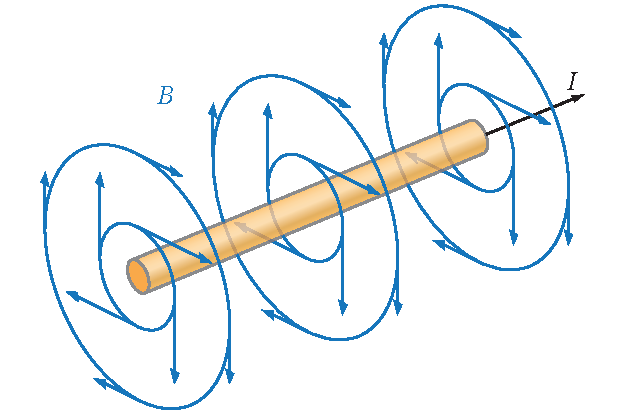
\includegraphics[width=0.5\textwidth]{fig-fio} 
\end{figure}


%\end{minipage}
%

%No sistema SI, a unidade de $\vec{B}$ é o Tesla (T).
%\footnote{No sistema SI, a unidade de $\vec{B}$ é o Tesla (T).} %N·A^{−2}
%\hspace{0.2cm}

%
%\begin{minipage}[b]{0.45\linewidth}
%\end{minipage}
No caso de uma espira\footnote{Termo que designa um circuito eléctrico fechado} circular, é criado um campo magnético cujas linhas de força são curvas fora do seu eixo e lineares apenas ao longo do eixo. Pode provar-se que o campo magnético criado por uma espira de raio $r$, percorrida por uma corrente de intensidade $I$, tem linhas de força fechadas\footnote{Mesmo aquelas que só \emph{fecham} no infinito}, ao contrário das linhas de força eléctricas. Isto coloca em evidência que $\vec{B}$ nos pontos do plano da espira, mas exteriores a esta, é antiparalelo a $\vec{B}$ no eixo da espira (ver figura). O módulo de $\vec{B}$ num ponto do eixo é dado por
\begin{equation}
	|\vec{B}_{\mathrm{fig5-espira}}| = \frac{\mu_0 I}{2 r} \sin^3 \alpha
\end{equation}

 \begin{figure}[h]
  \centering 
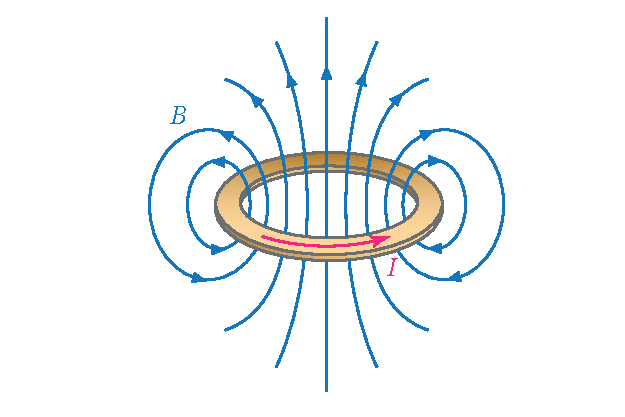
\includegraphics[width=0.5\textwidth]{fig-espira.pdf}
\end{figure}


\newpage
\section{Figuras dos aparelhos da montagem experimental}
\begin{figure}
	[htb]  \centering 
	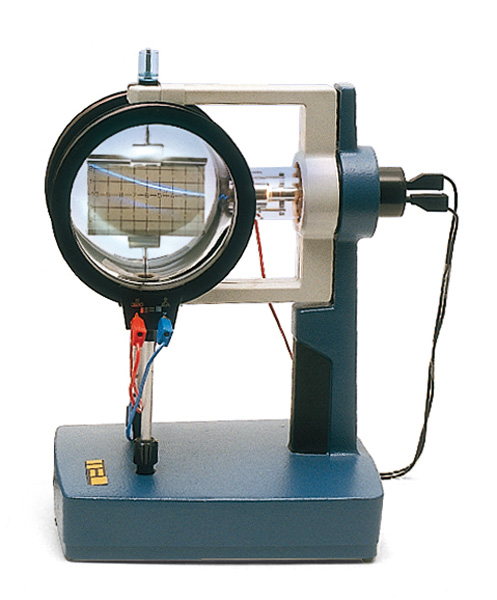
\includegraphics[width=0.45\textwidth]{./fig3-ThomsomEquip}
	\caption{Montagem da Experiência de Thomson com tubo de raios catódicos, suporte e par de bobines de Helmholtz. \label{fig:Thomson_Equip}} 
\end{figure}

\begin{figure}
	[hb]  \centering 
	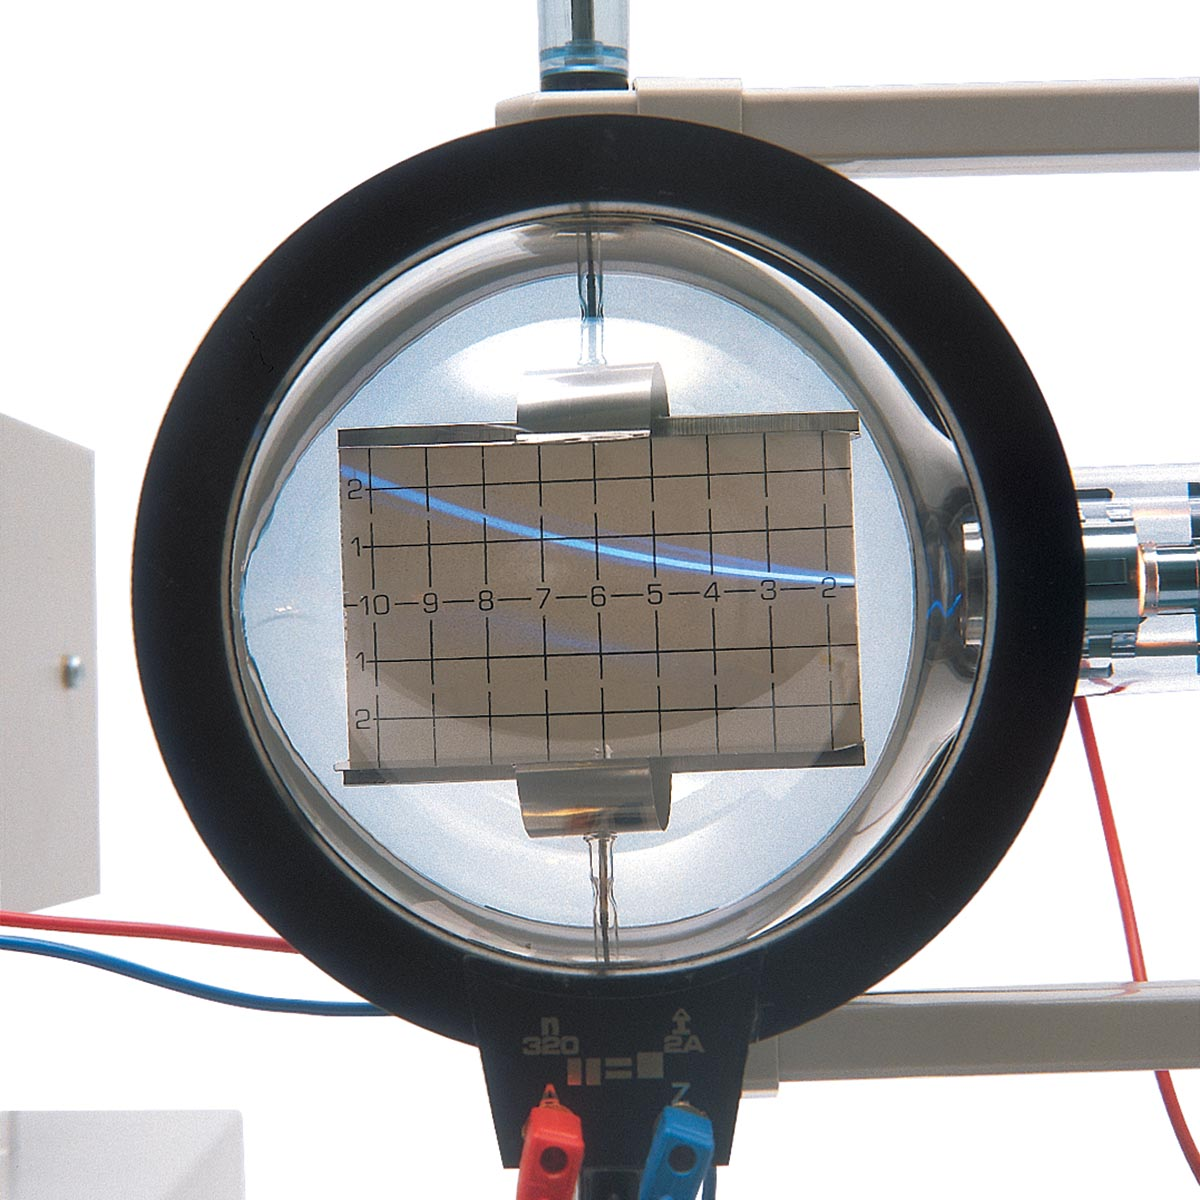
\includegraphics[width=0.4\textwidth]{./fig4-Thomson_Electron-Deflection-Tube-D}
	\caption{Trajectória dos electrões sujeitos a um campo magnético perpendicular. \label{fig:Thomson_trajec}} 
\end{figure}

\newpage

\section{\sf Procedimento Experimental}
{ \large Material }
\begin{itemize}
	\item Ampola (tubo) de raios catódicos (TRC), modelo TEL 525.
	\item 	Fonte de alimentação do TRC, que inclui alimentação de alta tensão contínua 
	(até 5000 V) aplicada aos eléctrodos (cátodo e ânodo) do TRC e alimentação de baixa tensão
	(6.3 V AC) para o filamento do TRC.
	\item Par de bobinas que envolvem a parte esférica do TRC na configuração de
	Helmholtz (para criar um campo magnético aproximadamente homogéneo na
	região central entre as bobinas, de raio médio $r$, e afastadas de $r$ uma da outra).
	\item Fonte de alimentação de corrente \textbf{contínua} (em modo DC) para as bobinas.
	\item Multímetro (como amperímetro) a instalar em \textbf{série} no circuito das bobinas.
\end{itemize}

O tubo TRC tem um filamento alimentado por 6.3 V (em modo AC). Este filamento emite electrões por efeito termiónico. 
Entre o ânodo e o cátodo do tubo estabelecem-se diferenças de potencial $ (V_+ - V_-) = U_a$ . Os electrões são acelerados entre o cátodo e o ânodo e a sua velocidade à saída do ânodo é função de $U_a$. 

Ao entrarem na parte esférica do tubo, os electrões podem ser deflectidos por \emph{campos magnéticos} provocados por correntes que percorrem as bobinas de Helmholtz e/ou por \emph{campos eléctricos} devidos à aplicação de tensão entre duas placas paralelas ligadas aos pontos 1 e 2 do diagrama (Fig. \ref{fig:TL}).

O campo de indução magnética $B$ devido às bobinas de Helmholtz é aproximadamente uniforme na região central entre as bobinas, e para uma corrente $I$ é dado por\footnote{No sistema SI, a unidade de campo magnético é o Tesla (T), sendo 1\,T=1\,Weber/m$^{2}$ .}:
\begin{align}
	\label{eq:helmotz}
	 n &= 320\textrm{ espiras} \nonumber \\ 
B = \left(\frac{4}{5}\right)^{3/2} \cdot \frac{\mu_0 n I}{r} =  \frac{32 \pi n }{5 \sqrt{5}} \cdot \frac{I}{r} \cdot 10^{-7}\textrm{ Weber/m}^{2}
 \qquad  r  &= 0.068\textrm{ m} \\
r  &= d/2 \nonumber
\end{align}

\begin{figure}
	[h]  \centering 
	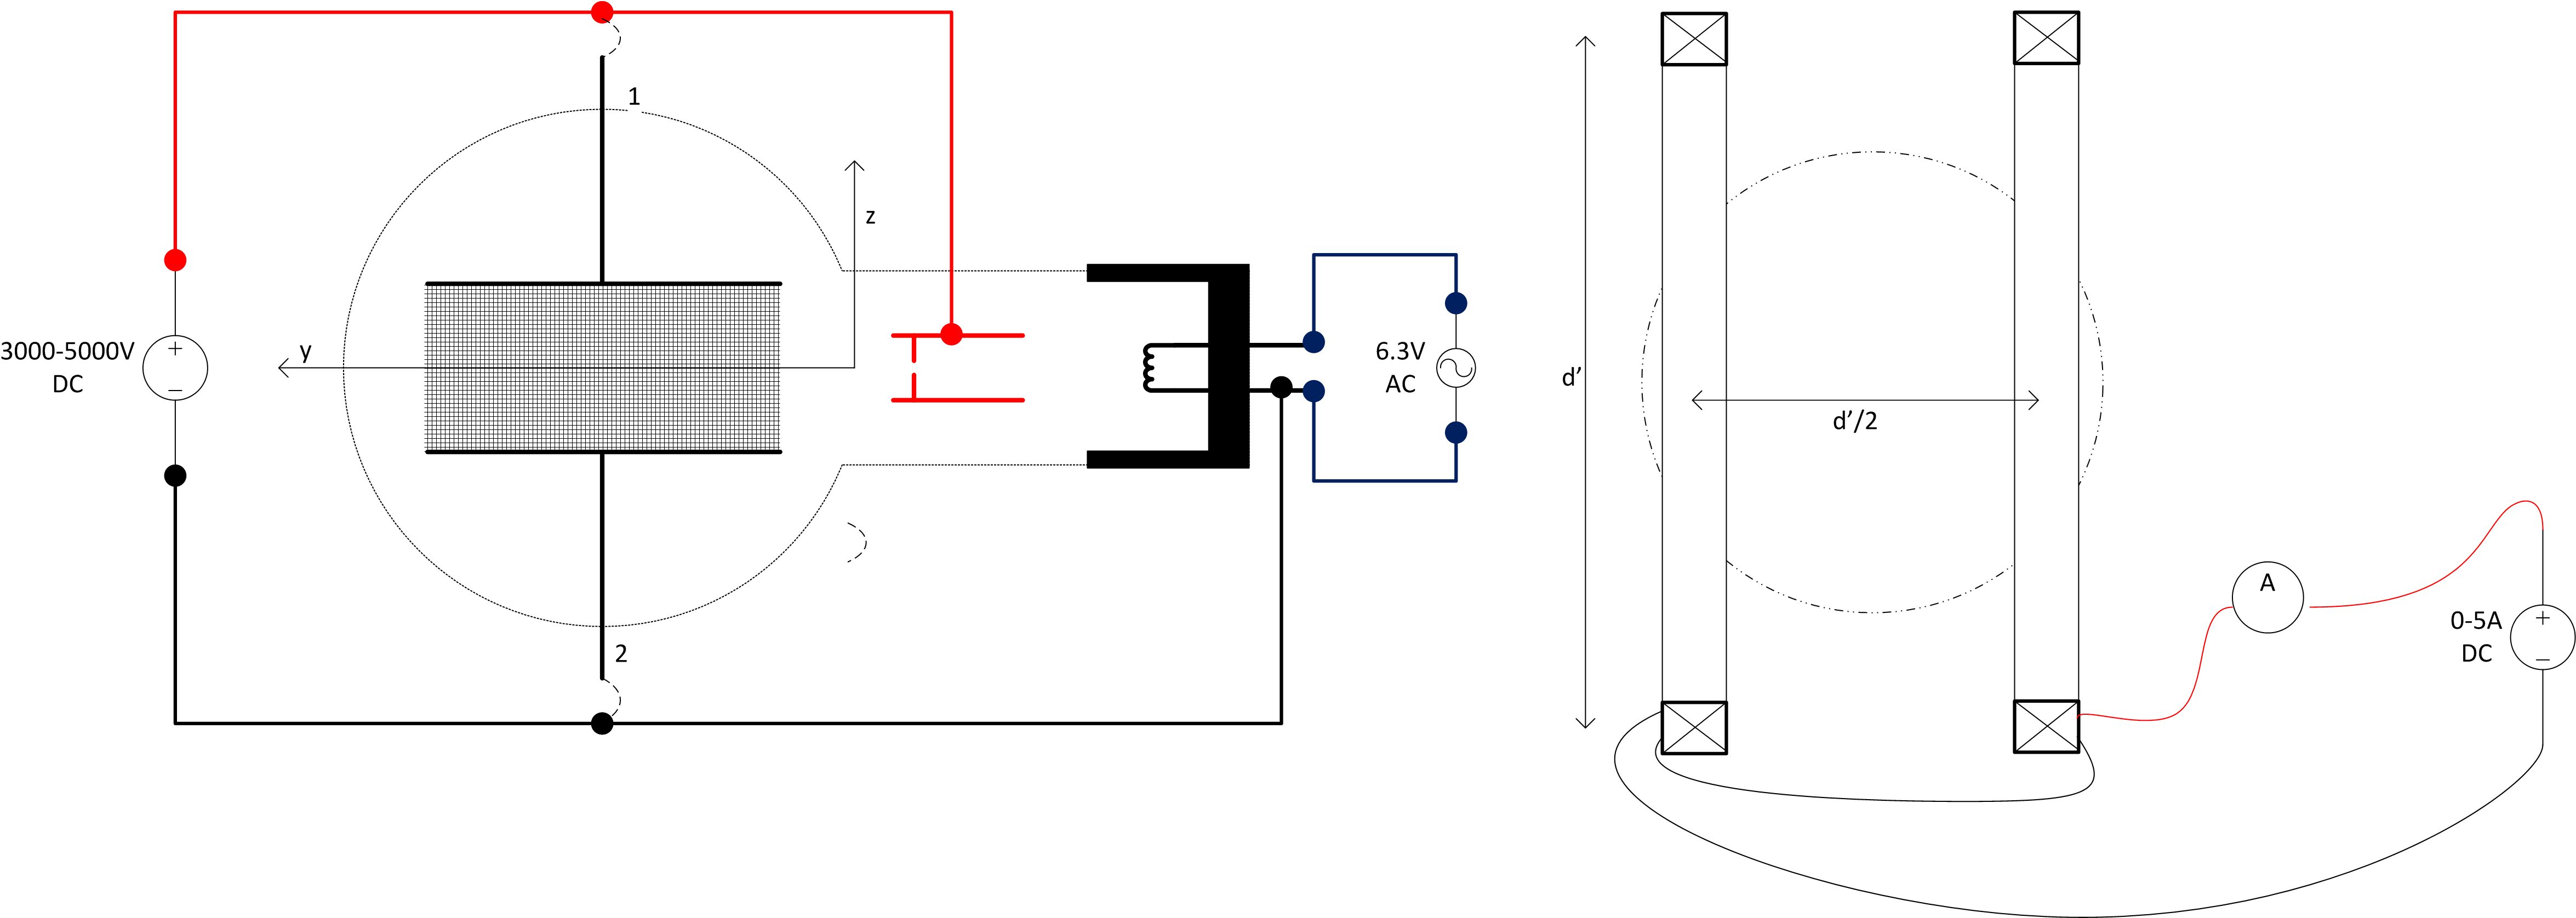
\includegraphics[width=0.8\textwidth]{fig5-TuboTL} 
	\caption{Diagrama do tubo utilizado e geometria das bobinas de Helmholtz \label{fig:TL}} 
\end{figure}

\subsection{\sf DETERMINAÇÃO DE $q/m$ POR  DEFLEXÃO MAGNÉTICA}
\subsubsection{\sf Trajectórias de partículas carregadas sujeitas a um campo magnético constante}
Quando se aplica uma tensão $U_a$ entre o ânodo e o cátodo (sem aplicar tensão entre os pontos 1 e 2 representados na Fig. \ref{fig:TL}), pode admitir-se que a velocidade final $v$ dos electrões ao abandonarem o ânodo é dada pela seguinte expressão 

\begin{equation}
	\label{eq:encin}
q\, U_a = \frac{1}{2} m \, v^2
\end{equation}
em que $q$  é a carga do electrão e $m$ a sua massa.

Ao chegarem à parte esférica do tubo os electrões são deflectidos pelo campo magnético $\vec{B}$ (com $\vec{B}\perp\vec{v})$ e a sua trajectória é circular de raio $R$, verificando-se:
\begin{equation}
	\label{eq:encin2}
B \, q\, v = \frac{m\,v^2}{R} 
\end{equation}
As trajectórias dos electrões podem ser visualizadas numa escala graduada feita de material fluorescente. 
A origem do reticulado está situada aproximadamente no início da zona 
sujeita ao campo $\vec{B}$.
Combinando (\ref{eq:encin}) e (\ref{eq:encin2}) obtém-se uma expressão para a relação $q/m$:
\begin{equation}
	\label{eq:encin3}
 \frac{q}{m} = \frac{2\, U_a}{B^2\,R^2} 
\end{equation}
em que:
\begin{description}
\item[$U_a$] – impõe-se e mede-se diretamente no voltímetro da fonte.
\item[$B$] – calcula-se para a corrente $I$ a partir da expressão (\ref{eq:helmotz}).
\item[$R$] – determina-se por leitura no écran fluorescente, das coordenadas de posição $y$ (horizontal) e $z$ (vertical) de pontos do feixe. Por construção do tubo verifica-se:
\begin{equation}
	\label{eq:eR}
 R = \frac{y^2 + z^2}{2 \, z} 
\end{equation}
\end{description}



\subsubsection{\sf Modo de proceder}


\begin{enumerate}
	\item Montar os circuitos eléctricos de acordo com a  Figura \ref{fig:TL} 
	(\emph{não os ligue antes de serem verificados pelo Docente!}).
	\item Observe qual é o valor máximo de tensão no gerador de  alta tensão que dispõe. Escolha esse valor.
	\item Ajustar a corrente das bobinas de Helmholtz $I_+$ de modo a que a circunferência passe por um ponto bem determinado\footnote{Utilize de preferência os maiores valores possíveis para o raio $R$, de forma a que o feixe se encontre na zona central entre as bobines.}.  Calcule $R$.
	Inverta o sentido da corrente e determine um novo $I_-$ para o mesmo raio $R$.
	Tomando $I_{\textrm{medio}} = (I_+ + I_-)/2 $ calcule o campo magnético $B_{\textrm{medio}}$. Utilize a semi-diferença, $(I_+ - I_-)/2$, para a estimativa das incertezas $\delta I_{\textrm{medio}}$ e $\delta B_{\textrm{medio}}$.
	\item Repita o ponto 2) para quatro novos valores de $R$. 
	\item Repetir 1), 2) e 3)  e para os mesmos $R$, para dois valores inferiores de tensão, afastados por exemplo de 500 V entre si.
	\item Apresente os valores de $q/m$ para os 15 ensaios. Calcule a média desses valores para cada $R$, assim como a incerteza da média.
	\item Para um ensaio estime a contribuição relativa das incertezas das grandezas que mediu para a incerteza total. Compare este erro assim calculado com a incertezas calculadas anteriormente.
	%Apresente para cada raio o valor de $q/m$ assim como o erro associado a cada uma das determinações. Compare e comente os resultados.
	\item Apresente um valor final para $q/m$. Estime a precisão e a exatidão obtida nas determinações que realizou.
\end{enumerate}
 
\subsection{\sf DETERMINAÇÃO DE $q/m$ POR DEFLEXÃO\\ MAGNÉTICA E ELÉCTRICA QUASE COMPENSADA }

\subsubsection{\sf Situação de equilíbrio entre as interacções eléctrica e magnética}
Uma carga q animada de uma velocidade $\vec{v}$ numa região em que existe um campo de indução $\vec{B}$ e um campo eléctrico $\vec{E}$ fica submetida a uma força de Lorentz\footnote{Se a força for apenas de origem magnética, $\vec{F}_m =  q\,(\vec{v} \times \vec{B})$, pode chamar-se também de \emph{Laplace}} $\vec{F}$ dada por:
\begin{equation}
	\label{eq:Lorentz}
 \vec{F} = q\; \vec{E} + q\,(\vec{v} \times \vec{B})
\end{equation}

Se as duas forças se equilibrarem -- ou seja, se forem de igual módulo e de sentidos opostos -- a carga $q$ não é desviada da sua trajectória. No nosso caso, em que $\vec{B} \perp \vec{v}$ , a condição de equilíbrio é dada por:
\begin{equation}
	\label{eq:equil}
 |\vec{E}| = v\, |\vec{B}|
\end{equation}

\subsubsection{\sf Montagem a efetuar}

Aproveitando a montagem já efectuada no ponto anterior, ligue agora os terminais 1 e 2 (Fig. \ref{fig:TL}) à fonte de alta tensão que gera a tensão $U_a$, produzindo assim na região do écran fluorescente um campo eléctrico. Fazendo com que as bobinas sejam percorridas por uma corrente com intensidade e  ``sentido'' convenientes, podemos obter uma força de origem magnética anti-paralela à provocada pelo campo $\vec{E}$. 
Deste modo, a trajectória visualizada no écran será aproximadamente retilínea, sendo a condição de equilíbrio dada por (\ref{eq:equil}):

\begin{equation*}
	%\label{eq:equil2}
 |\vec{E}| = v\, |\vec{B}| = \frac{U_a}{d} \qquad  \qquad  \textrm{(\ref{eq:equil}a)}
\end{equation*}
onde $d$ é a distância entre as placas do écran fluorescente e $U_a$ a tensão entre as mesmas, que é como se disse igual à tensão de aceleração.

A equação (\ref{eq:equil}a) permite-nos calcular a velocidade dos electrões, uma vez que podemos conhecer os valores de todas as outras variáveis aí intervenientes. O conhecimento de $v$ permite-nos calcular $q/m$ tendo em conta que, segundo (\ref{eq:encin}), deverá ser:

\begin{equation*}
%	\label{eq:encin}
\frac{q}{m} = \frac{v^2}{2} \; \frac{1}{U_a} \qquad \qquad \qquad  \textrm{(\ref{eq:encin}a)}
\end{equation*}

Ou finalmente, por combinação com (\ref{eq:equil}a):
\begin{equation}
%	\label{eq:encin}
\frac{q}{m} = \frac{1}{2} \; \frac{U_a}{B^2\; d^2} 
\end{equation}

\subsubsection{\sf Modo de proceder}
\begin{enumerate}
	\item Para cada uma das quatro tensões de trabalho $U_a$ já referidas, aplicadas agora também às placas que produzem o campo eléctrico, determine o valor de $B$ (a partir de $I$) que conduz ao anulamento das forças de origem eléctrica e magnética.
	\item Inverta o sentido dos campos eléctricos e magnéticos e repita a determinação do valor de $B$.
	\item Apresente os valores de $q/m$. Analise as diferentes contribuições para a incerteza total. Estime o valor da relação carga/massa do electrão, assim como a precisão e a exatidão obtida nas determinações que realizou.
	\item  Observe  a  trajectória  quando  as  forças  de 
origem eléctrica e magnética não se compensam. Comente. 
%	Apresente os valores de q/m calculados assim como o erro associado a cada determinação. Apresente um valor final para $q/m$.
\end{enumerate}

\end{document} 	
